The basic color of the website is white and a serious orange. The main background of the website is white, since it makes the view clear and simple which would comfort the users. According to research, this warm color orange is stimulating, not only stimulating emotions but also appetite\footnote{[ http://desktoppub.about.com/cs/colorselection/p/orange.htm ]}. Therefore, in order to make the website stand out and unique, the logo would be orange as well.

\subsection{Version 1}

\begin{figure}
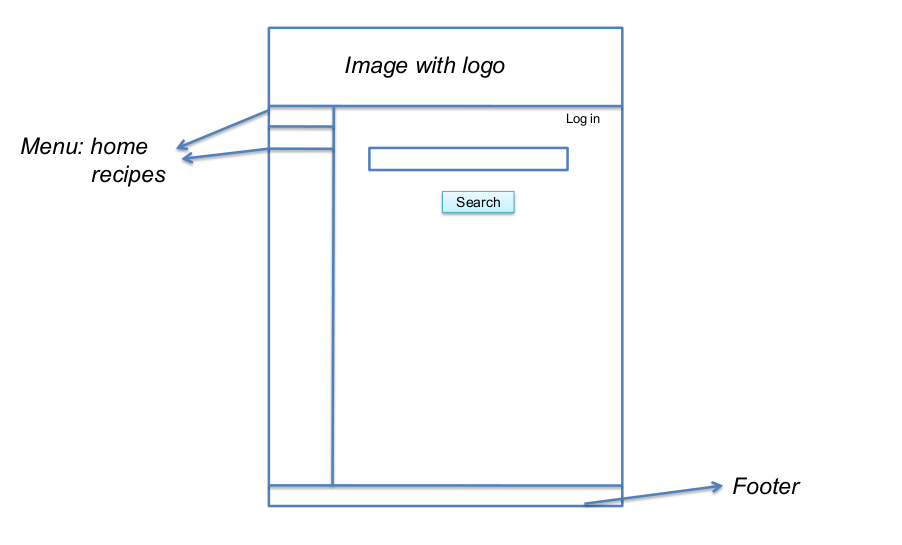
\includegraphics[width=0.9\textwidth]{home_page}
\caption{Layout of the Home Page}
\label{fig:home_page}
\end{figure}

Digichef is a with a web interface base on a web framework. Upon accessing the website, (Fig~\ref{fig:home_page}) users are presented there are three drop-down menus which allows people to select ingredients. The drop-down menus are transverse because the ingredients are related. After the user selected three ingredients and clicked on search, the page will be substituted to the page of recipe list. If the button “recipes” from the sidebar is clicked, moreover, the page will change to the whole list of all recipes ordering by alphabet.

\begin{figure}
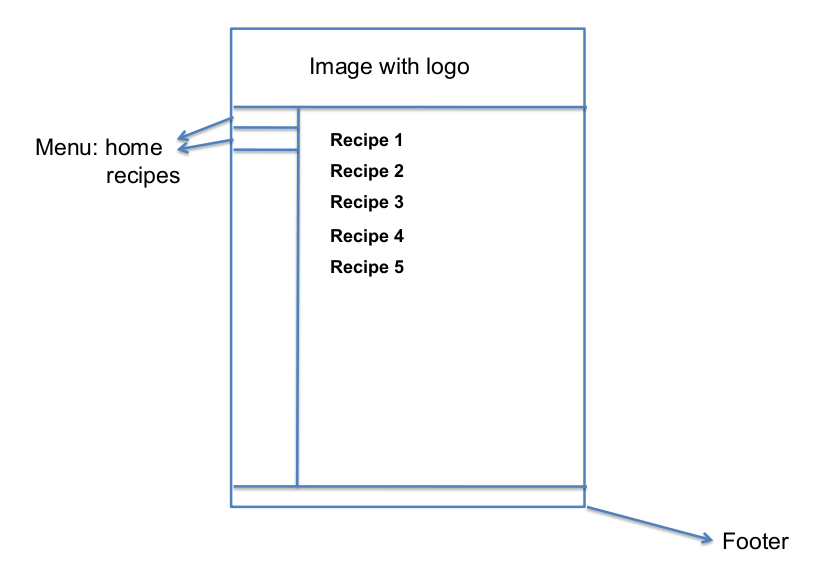
\includegraphics[width=0.9\textwidth]{recipe_list_page}
\caption{Layout of the Recipe List Page}
\label{fig:recipe_list}
\end{figure}

The recipe list page (Fig~\ref{fig:recipe_list}) contains a list of recipes with at least one of the three ingredients. In each recipe, other ingredients would be included as well, nevertheless. Once one recipe is selected, the web will connect to the exact recipe page.

\begin{figure}
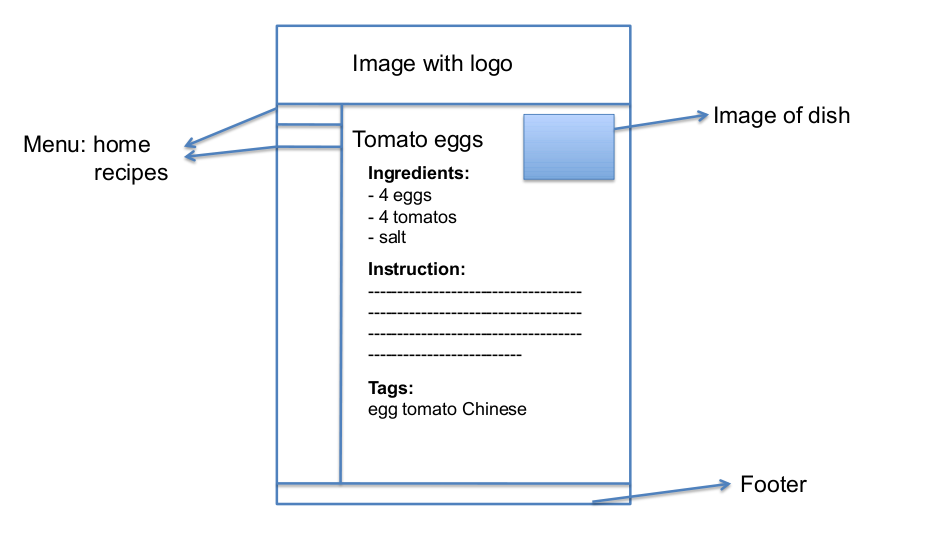
\includegraphics[width=0.9\textwidth]{recipe_page}
\caption{Layout of the Recipe Page}
\label{fig:recipe_page}
\end{figure}

The recipe page (Fig \ref{fig:recipe_page}) contains the details of the recipe, recipe name, ingredients, the instruction, and tags. The tags are mainly about the ingredients of the recipe and the region of the recipe.
One of the basic limitation of version 1 is that the website only has three drop-down menu for the user, that is, the user could not type in ingredients. The reason we only have three drop-down menus at this point is that the version 1 is quite small, and we also only have limited number of recipes. Therefore, for version 2, the home page will have three text-fields instead. Furthermore, the web interface is also need to be more clear and attractive in the future.

\subsection{Version 2}
Version 2 is an upgraded version of the original version containing more functions ( as shown in the Product Specification). With the use of JAVAScript, the web interface will be more professional and attractive. Users, moreover, could enter text data regarding their ingredients into a text box which uses tab completion instead of using a drop-down menu. There will also be a larger database of ingredients hence justifying the use of tab completion as apposed to a drop-down menu.
Additionally, for version 2, users are allowed to create their own account. With this account, a user can have their own history of recipes that they rate. Each recipe would be rated from 1 star to 5 stars. Additionally, the home page will contain not only the area for search of recipes but also the area made of brief look of the most popular recipes. And once the user has logged in, the home page will also have an area that gives suggest recipes based on past rating. 
One typical improvement for the home page is that, the search-text-field allows user to search by combination of ingredients. Thus, user could search recipes by typing multiple ingredients separated by commas or spaces. And the result of the recipe list is ordered according how matching the ingredients are. 
For the recipe page, with the image of the recipe, a new area called “You might like” would be also added.  This area is also made up of a list of brief look of recipes. These recipes are chosen from the database using collaborative filtering techniques. In addition, users, at this point, could click the tags and get a list of recipes that contains this tag.
The last but not the least, we will also have a simple web view for mobile phone and other portable equipment (iTouch, psp, etc). This mobile view is only simple black and white appearance with the same function as the version 1, which could be accessed through the internet.

\subsection{Version 3}
The ideal version, which is the third version of digichef, would not only have a more friendly website based on version 2 but also a mobile application that user could actually install. And the recipes are searchable by more than ingredients, for instance, the region of this recipe (Chinese dish) or other category like vegetarian. 
With the increasing of the whole database and tag system, the home page would also have the area contains the most popular tags. When the user click on a typical tag, the website would update with a list of recipes which ordered by rates. 
Once the user want to rate recipe, the webpage would open a feedback dialog box which allows user to rate it vary from one star to five stars, and also allows user to leave their own command about this recipes. And a number of the latest command would be showed on the exact recipe page. 
A huge improvement of version 3 is that user could upload their own recipes. When they construct the new recipe, they need to provide the name, the ingredients, the instruction and also the tag to classify the recipe. Thus, the new version of recipe page would be same as version 2 but with author’s name. 

